\documentclass[11pt,a4paper]{article}
\usepackage{amsmath,amsthm,amssymb}
\usepackage{parskip}
\usepackage{listings}
\lstloadlanguages{R}
\usepackage{verbatim}
\usepackage[usenames,dvipsnames]{color}
\usepackage{esdiff}
\usepackage{subfig}
\lstset{
   language=R,
   basicstyle=\ttfamily,
   columns=fixed,
   fontadjust=true,
   breaklines=true,
   basewidth=0.5em,
   keywordstyle=\color{blue},
   commentstyle=\color{ForestGreen},
   stringstyle=\color{mauve}
}
\fontfamily{cmr}
\usepackage[margin=1in, tmargin=0.75in, bmargin=0.75in]{geometry}
\usepackage{graphicx}
\usepackage{enumerate}
\title{MAS212 Assignment 3:\\Numerical methods for solving ODEs:\\Accuracy, stability and stiffness}
\author{140185164}
\date{}
\begin{document}
\maketitle
\date{}
In this assignment we have been tasked with investigating the various ways in which one can produce numerical approximations to a system of ODEs. With numerical approximations comes inaccuracies and instabilities, so we will  investigate the effect that these have on the approximations.

\subsection*{The midpoint method}
We are given an equation for damped harmonic motion:
\begin{equation}\ddot{u}+2\dot{u}+5u=0.\end{equation}

It can be shown that $u(t) = Au_1(t) + Bu_2(t)$ is a solution to a second order linear homogeneous ODE if $u_1(t)$ is a solution and $u_2(t)$ is a solution.$^{[1]}$ If we make a guess that $e^{\lambda t}$ is a solution to our ODE, for some $\lambda \in \mathbb{R}$, then by substituting into (1) we get:
\begin{align*}
\text{LHS}&=\diff[2]{}{t}e^{\lambda t} + 2\diff{}{t}e^{\lambda t} +5e^{\lambda t}
	       =\lambda ^2 e^{\lambda t} +2\lambda e^{\lambda t} +5e^{\lambda t} 
	       =e^{\lambda t} \big(\lambda^2 +2\lambda +5\big)=0.\\
\end{align*}
By the properties of the \textit{exponential} function, $e^{\lambda t }\neq 0$, and so $\lambda^2 +2\lambda +5=0$ (\textit{Auxillary Equation}). Solving this equation gives $\lambda = {-1}\pm 2i $, and so we can see that $\lambda=\{{-1}+2i,{-1}-2i\}.$ We have two solutions to the \textit{Auxillary Equation} and by the theorem above, we have the general solution
 \begin{align*}u(t)=&Ae^{({-1}+2i)t}+Be^{({-1}-2i)t}=e^{{-t}}\big(Ae^{2i}+Be^{{-2}i}\big)\\
=&e^{{-t}}\big(A\cos(2t)+Ai\sin(2t)+B\cos(-2t)+Bi\sin(-2t)\big)\\
=&e^{{-t}}\big((A+B)\cos(2t)+ (Ai-Bi)\sin(2t)\big)\\
=&e^{{-t}}\big(C\cos(2t)+D\sin(2t)\big)
\end{align*}
by the application of \textit{Euler's Theorem}, where $C=A+B$ and $D=Ai-Bi$.
To find the particular solution, we are given that $u(0)=1 \implies e^{{0}}\big(C\cos(0)+D\sin(0)\big)=C=1$, so now $u(t)=e^{{-t}}\big(\cos(2t)+D\sin(2t)\big).$ Differentiating $u(t)$ with respect to $t$ gives \\$\dot{u}(t) = -e^{{-t}}\big(\cos(2t)+D\sin(2t)\big) + e^{{-t}}\big({-2}\sin(2t) +2D\cos(2t)\big).$ Our other initial condition is that $\dot{u}(0)=0\implies -e^0\big(1+0D\big)+e^0\big({-2}(0) +2(1)(D)\big)={-1}+2D=0 \iff D=\frac{1}{2}.$ Therefore, our particular solution is given by \begin{equation}\overline{u}(t)=e^{-t}\Big(\cos(2t)+\frac{1}{2}\sin(2t)\Big).\end{equation}

\par
Next I plotted a time-domain plot and a phase portrait for equation (2) in \textit{Python} in the domain $t \in [0,4]$ as an exact solution, and also solved the coupled differential equations\\ $\dot{u}=v, \ \dot{v}={-2v}-5u$ numerically by the midpoint method. The plots are shown in Figure 1.

\begin{figure}[h]
\caption{Time-domain plot and a phase portrait for equation (2) for initial conditions $u_0=1$ and $v_0=0$}
\centering
\subfloat[Time-domain graph] {
	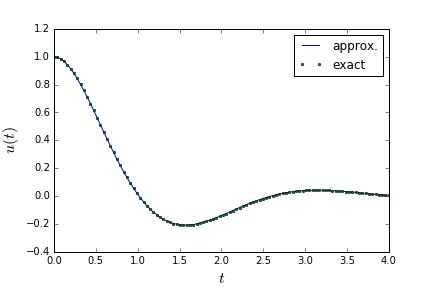
\includegraphics[scale=0.45]{1a_time-dom.jpg}
	}
\hfill
\subfloat[Phase portrait] {
	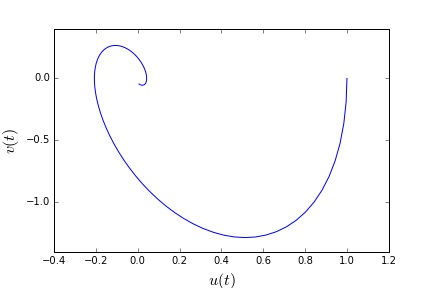
\includegraphics[scale=0.45]{2a_phaseplot.jpg}
	}
\end{figure}

Figure 1(A) shows us a time-domain graph with both the midpoint method approximation of $u(t)$ and the exact solution of $u(t)$ for $t \in [0,4]$. I used 102 intervals between $t_0$ and $t_4$, and so the midpoint method shows solutions that lie very close to the line giving the exact solution of $u(t).$ However, by zooming into the graph to show a very small section of the time-domain plot, it is possible to see that the approximations do not lie exactly on the exact solution plot, and so the midpoint method gives us some errors against the exact solution. The phase plot shows what appears to be a spiral forming over our given time-domain and it does not appear to be converging to a limit cycle in this time. 

\subsubsection*{Accuracy}
The midpoint method can be shown to be second-order accurate, meaning that its global truncation error scales with $h^2$, where we have defined $h$ as the step size between each interval in the time-domain we approximated over. One way to illustrate this is to create a so called \text{log-log plot} of $h$ against error $\epsilon$ given by $\epsilon=\sqrt{(u-\overline{u})^2+(v-\overline{v})^2}$.  Here, $u$ and $v$ are the approximations to the coupled differential equations, and $\overline{u}$ and $\overline{v}$ are the analytic solutions of the particular solution ($u$ and $\diff{u}{t}$ respectively) at a given value of $t$. 

We were asked to evaluate the error at $t_2$ for a number of different valules of $h$. For $u(2)$ and $v(2)$, it wasn't guaranteed that for every step size that there would be an approximation at exactly $t_2$, and so I used a function in python to interpolate the values $u(2)$ and $v(2)$ from the data points that \textit{had} been approximated. The error at $t_2$ for each step-size $h$ were then calculated and plotted, with the axes scaled logarithmically. The plot is shown below.

\begin{figure}[h]
\caption{Graph plotting step size $h$ against error $\epsilon$ at time $t_2$ on logarithmic axes}
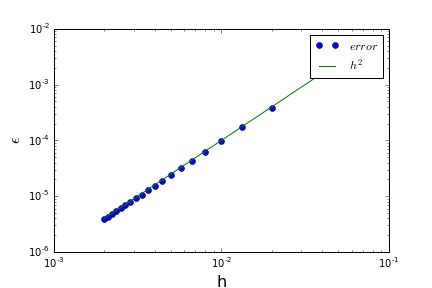
\includegraphics[scale=0.6]{error.jpg}
\centering
\end{figure}

As well as plotting the error points on the graph in Figure 2, there is a green line representing the points $(h,h^2)$. All of the error points plotted on the graph are plotted very close to the line representing $(h,h^2)$, which shows that error $\epsilon$ scales with $h^2$, for our points $h<<1$.


\section*{Stability and Stiffness}
I will now investigate the notion of stiffness and stability which occur in the numerical approximations of some ODEs. We will be investigating these themes using the coupled differential equations: \begin{align*}\dot{u}=&(b-2a)u+2(b-a)v\\
\dot{v}=&(a-b)u+(a-2b)v, \qquad u(0)=1,\ v(0)=0.
\end{align*}
Firstly we will derive the analytical solutions to our system of equations. We are given that $u=2y-z$ and $v=-y+z$, where $y$ and $z$ are derivatives with respect to $t$ (solving these two equations simultaneously gives that $y=u+v$ and $z=u+2v$ - we will need this later). By the chain rule we can show that $\diff{u}{t}=\frac{\partial u}{\partial y}\diff{y}{t}+ \frac{\partial u}{\partial z}\diff{z}{t}=2\dot{y}-\dot{z}$ and \\$\diff{v}{t}=\frac{\partial v}{\partial y}\diff{y}{t}+\frac{\partial v}{\partial z}\diff{z}{t}=-\dot{y}+\dot{z}=$, and by substituting for $u,\ v,\ \dot{u}$ and $\dot{v}$ into the system of equations we get:
\begin{align*}
2\dot{y}-\dot{z}&=(b-2a)(2y-z)+2(b-a)(-y+z),\\
-\dot{y}+\dot{z}&=(a-b)(2y-z)+(a-2b)(-y+z) \end{align*}
\begin{equation}\iff 2\dot{y}-\dot{z}=bz-2ay, \end{equation}
\begin{equation}-\dot{y}+\dot{z}=ay-bz \end{equation}
We can reduce these two equations into functions of only two variables by carrying out $(3)+(4)$ and $(3)+(2\times (4))$ to give
$$\dot{y}=-ay, \qquad \dot{z}=-bz.$$
Remembering that $\dot{y}=\diff{y}{t}$ and $\dot{z}=\diff{z}{t}$, by the method of seperation of variables we can solve these first order ODEs to get 
\begin{equation}y=u+v=Ae^{-at},\end{equation}
\begin{equation}z=u+2v=Be^{-bt}.\end{equation}
Finally by performing $(6)-(5)$ and $2(5)-(6)$ we get $u(t)=2Ae^{-at}-Be^{-bt}$ and \\$v(t)=Be^{-bt}-A^{-at}.$ 
Plugging in our initial conditions, $u(0)=2A-B=1$ and $v(0)=B-A=0$ implies that $A=B=1$. Therefore we have our particular solutions:
\begin{align*}
\overline{u}(t)&=2e^{-at}-e^{-bt}\\
\overline{v}(t)&=e^{-bt}-e^{-at}.
\end{align*}


For the following plots, we will take $a=1$ and $b=200$.
The next task is to plot time-domain plots graphing exact solutions $\overline{u}(t)$ and $\overline{v}(t)$ against time, alongside approximations to $u(t)$ and $v(t)$ for different $h$ values against $t\in[0,1]$. See Figure 3 and Figure 4 to find four plots respectively for the interval step-sizes $h=\{0.0025,0.005,0.01,0.02\}$.

\begin{figure}[h]
\caption{Four time-domain plots for the given $h$ values for time $t$ against $u(t)$.}
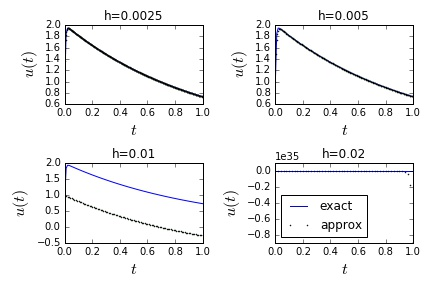
\includegraphics[scale=0.8]{t_ut_sub.jpg}
\centering
\end{figure}

Our four graphs in Figure 3 show that, for $h=0.0025$ and $h=0.005$, where $h$ is small enough, the midpoint method approximation of the differential equation of $\dot{u}(t)$ is plotted practically on top of the exact solution. This means that the midpoint method approximation gives only a very small error against the exact solution for the given time-domain. However, as the step size increases, our graphs for $h=0.01$ and $h=0.02$ show that the errors become much more prominent over our time interval. For $h=0.01$, we can see that the approximation of $u$ is approximately a translation of the exact solution by one unit parallel to the negative $y-axis$ for all $t$ values. For $h=0.02$, it is essential to notice that the $y-axis$ is scaled by a factor of $10^{35}$. For $t\in[0.9,1]$ we can see that the midpoint approximation of $u(t)$ decreases rapidly from around $u(0.9)\approx 0$ to $u(1)\approx {-0.2}\times 10^{35}$.

Next we can analyse the difference between the midpoint method approximation of $\dot{v}(t)$ and its exact solution. The four plots below show correspond to plots for the different $h$ values stated above.

\begin{figure}[h]
\caption{Four time-domain plots for the given $h$ values for time $t$ against $v(t)$}
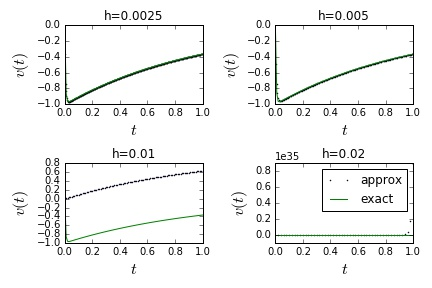
\includegraphics[scale=0.8]{t_vt_sub.jpg}
\centering
\end{figure}

For $v(t)$ a similar story unfolds. Midpoint method approximations for $v(t)$ with $h=0.0025$ and $h=0.005$ give approximations that give extremely small errors compared to the exact solution over our time-domain. The approximation for $h=0.01$ gives a translation of the exact solution, but this time by one unit parallel to the positive $y-axis$, and the approximation for $v(t)$ for $h=0.02$ gives a sharp increase in $v(t)$ between $t=0.9$ and $t=1$, specifically an increase from $v(0.9)\approx 0$ to $v(1)\approx 0.2\times 10^{35}.$

Our analysis of the eight plots above show that as $h$ increases, the midpoint method approximations for $u(t)$ and $v(t)$ become very unstable for some values of $t$, so to keep the midpoint method as accurate as possible it is advisable to make $h$ sufficiently low.

\subsubsection*{Matrix form}
It is possible to show the equations
\begin{align*}
u_{n+1}&=u_n+h[(b-2a)u_{n+1}+2(b-a)v_{n+1}],\\
v_{n+1}&=v_{n}+h[(a-b)u_{n+1} +(a-2b)v_{n+1}]
\end{align*}
in the form $\boldsymbol{Ax}_{n+1}=\boldsymbol{x}_n$, with $\boldsymbol{A,\ x}_n$, and $\boldsymbol{x}_{n+1}$ as defined in the assignment brief. I will show this below: 


\[\boldsymbol{Ax}_{n+1}=\begin{pmatrix}1+(2a-b)h& 2(a-b)h\\ (b-a)h & 1+(2b-a)h\end{pmatrix}\begin{pmatrix} u_{n+1}\\ v_{n+1}\end{pmatrix}\]
\[= \begin{pmatrix}u_{n+1}+(2a-b)hu_{n+1} + 2(a-b)hv_{n+1}\\ (b-a)hu_{n+1}+v_{n+1}+(2b-a)hv_{n+1}\end{pmatrix}.\]
If we rearrange the implicit equations for $u_{n+1}$ and $v_{n+1}$ in terms of $u_n$ and $v_n$, and express them in terms of a column vector we get
\[\boldsymbol{x}_n =\begin{pmatrix}u_n\\v_n \end{pmatrix}= \begin{pmatrix}u_{n+1}-h[(b-2a)u_{n+1}+2(b-a)v_{n+1}]\\ v_{n+1}-h[(a-b)u_{n+1}+(a-2b)v_{n+1}]\end{pmatrix}\]
\[=\begin{pmatrix}u_{n+1}+(2a-b)hu_{n+1}+2(a-b)hv_{n+1}\\ v_{n+1}+(b-a)hu_{n+1}+(2b-a)hv_{n+1}\end{pmatrix},\]
which, it is easy to notice is equal to $\boldsymbol{Ax}_{n+1}.$ We have therefore shown that $\boldsymbol{Ax}_{n+1}=\boldsymbol{x}_n.$

\subsubsection*{Implicit Euler method}
\begin{figure}[h]
\caption{Time-domain plots for time $t$ against $u(t)$}
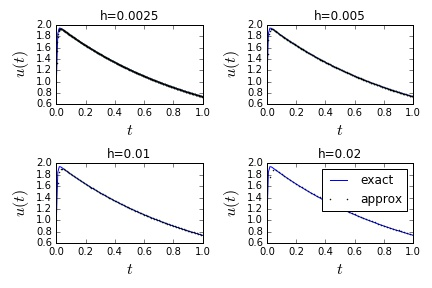
\includegraphics[scale=0.8]{back_euler_u.jpg}
\centering
\end{figure}
The \textit{implicit Euler method} is used for stiff ODEs. Our ODEs are stiff \textit{and} linear, and so by expressing the ODEs as a matrix equation, one can implement the \textit{implicit Euler method} by iteratively solving the matrix equation for $\boldsymbol{x}_{n+1}$. I did this for the step-sizes used previously, which were $h=\{0.0025,0.005,0.01,0.02\}$.
\begin{figure}[h]
\caption{Time-domain plots for time $t$ against $v(t)$}
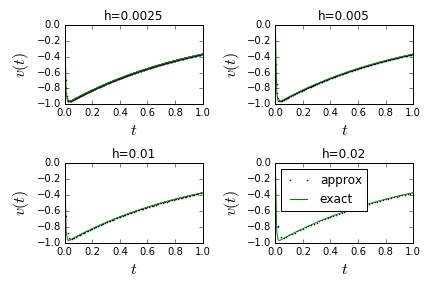
\includegraphics[scale=0.8]{back_euler_v.jpg}
\centering
\end{figure}
Figure 5 and Figure 6 show a small amount of error between the implicit Euler method approximations and the analytical solutions of $u(t)$ and $v(t)$ for our four values of $h$, but this is to be expected with all numerical approximations to a function. It is possible to reduce the error, and therefore increase the accuracy of numerical solutions by numerical methods by increasing the step-size $h$, as shown for $h=0.0025$ and $h=0.005$. 

However, unlike our approximations of the system ODEs with the midpoint method, the implicit Euler method does not show instability for higher values of $h$, or in our case, $h=0.01$ and $h=0.02$. The plots for these values of $h$ do not begin to diverge from the analytical solutions. This is evidence of a property of an implicit method in which they are stable for all $h$.

\subsubsection*{Implicit and explicit methods}
An \textit{implicit} method is a method where, for some sequence of $x_n$ values for $1\leq k < n$, $x_{k+1}$ is calculated by an equation containing $x_{k+1}$. The equation therefore contains $x_{k+1}$ on both sides. However, an \textit{explicit} method is a method by which $x_{k+1}$ is calculated by evaluating an expression not containing $x_{k+1}$. Therefore $x_{k+1}$ is expressed \textit{only} in $x$ terms not including $x_{k+1}$. 
If you require to solve an ODE that is non-stiff, or a stiff ODE that can be transformed somehow into a problem that isn't stiff, then an explicit method will work well to solve it for a sufficiently small $h$. However, if the ODE is stiff and there isn't a way to transform it into being non-stiff, then explicit methods encounter problems in evaluation, namely instabilities for relatively large $h$, and so an implicit method is used instead.$^{[2]}$ 

One example of an implicit method is the \textit{backwards Euler method} as seen previously in this report. Another implict method is the \textit{Trapezoidal rule} which is also used in computing solutions to ODEs. It can be classified as both a Runge-Kutta method and a linear multistep method.$^{[3]}$ One explicit method that we have also utilised in this report is the \textit{midpoint method}, also known as \textit{the second-order Runge-Kutta method}. Another explicit method is the \textit{forwards Euler method}; the Euler step in the forwards Euler method is utilised in the second-order Runge-Kutta method, which has an added step compared to the forwards Euler method for increased accuracy of solutions. 

In applying both explicit and implicit methods to this stiff ODE, I have learnt that, since our ODEs are linear, it is just as easy to implement an implicit method as it is to implement an explicit method, however I would use an implicit method where possible since it doesn't have the instability issues that explicit methods suffer from. Since there is no fixed step-size for which an explicit method becomes unstable for every ODE, it could become troublesome to determine whether your approximations to an ODE are accurate, if, for example, the ODE you are working with is non-linear. In this case you wouldn't have an analytical solution to compare your approximations to.

The second order Adams-Moulton (AM2) method is implicit, and, since a differential equation of $k^{th}$ order results in an accuracy of $k+1$, we can see that, for our system of ODEs, we would be numerically solving for $u(t)$ and $v(t)$ at second order accuracy. The AM2 method is given by:
$$y_{n+1}=y_n+\frac{h}{2}(f(y_{n+1},t_{n+1}+f(y_n,t_n)).^{[4]}$$

Throughout this report, I have been able to utilise both explicit and implicit techniques for approximating solutions to particular ODEs. In this study, I have found that explicit methods are useful for quickly computing a solution to a non-stiff ODE. However, as we found when studying our stiff system, explicit methods run into dire trouble when larger $h$ values lead to extreme errors compared to its analytic solution, and this was due to the instability of explicit methods for stiff ODEs. Here, implicit methods such as the backwards Euler method eradicated the instability for the larger $h$ values we used, and so we saw how incredibly useful implicit methods were in these situations.
\clearpage
\section{References}
[1]	Stewart,J. (2013) \textit{Second-Order Linear Differential Equations}. [online] [viewed 29$^{th}$ November 2015]. Available from: http://www.stewartcalculus.com/data/CALCULUS\%20Concepts\%\\20and\%20Contexts/upfiles/3c3-2ndOrderLinearEqns\_Stu.pdf

[2]	Baraff,D. (1997) \textit{Physically Based Modeling: Principles and Practice. Implicit Methods for Differential Equations}. [online]. Pittsburgh, Pennsylvania, Robotics Institute, Carnegie Mellon University [viewed $29^{th}$ November 2015]. Available from: https://www.cs.cmu.edu/~baraff/sigcourse/notese.pdf

[3]	Wikipedia (2015) \textit{Trapezoidal rule (differential equations)}. [online]. Wikipedia [viewed 3$^{rd}$ December 2015]. Available from: https://en.wikipedia.org/wiki/Trapezoidal\_rule\_\%28differenti\\al\_equations\%29

[4]	Zeltkevic,M. (1999) \textit{Adams Methods}. [online]. The Massachusetts Institute of Technology, Massachusetts [viewed on $3^{rd}$ December 2015]. Available from: http://web.mit.edu/10.001/Web\\/Course\_Notes/Differential\_Equations\_Notes/node6.html


\end{document}